                                                                         %\RequirePackage[l2tabu, orthodox]{nag}
%\documentclass[crop=false,parskip=half]{scrartcl}
\documentclass{article}
\usepackage[subpreambles=false]{standalone}
\usepackage{import}
\usepackage{preamble}
\usepackage{makeidx}
\makeindex


\begin{document}

\import{./}{title.tex}

\tableofcontents


\section{Schematic Diagram}\label{sec:PVTheory}
\begin{figure}[h]
\centering
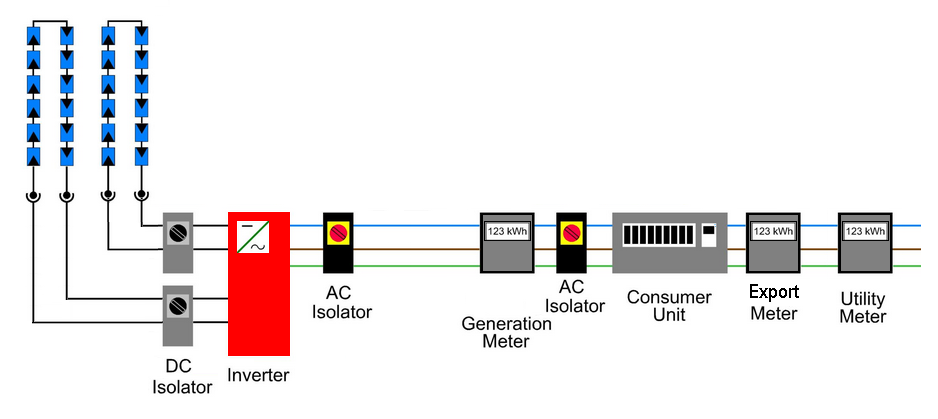
\includegraphics[width=\textwidth]{../figures/domestic-grid-tied-PV.png}
%\\[0.5]
\caption{Schematic of a domestic grid tied PV system}
\label{fig:domesticPV-schematic}
\end{figure}
\section{Equipment}
\begin{enumerate}
\item \textbf{Panels}
\begin{itemize}
\item	There are many manufacturers of panels but most people go with the big brands such as Sanyo, Sharp, Panasonic, BP Solar etc. 
\item	Data sheets for panels give information such as panel area, efficiency, $V_\text{OC}$, $I_\text{SC}$, $P_\text{max}$ at standard test conditions (\SI{1000}{\watt\per\metre\squared}, \SI{1.5}[AM]{}, \SI{25}{\celsius}), temp coefficient of power etc.
\item	Modules are generally connected in series with a number in series called a string. 
\item	The inverter may be able to cope with more than one string. All panels together are known as an array
\item	Connecting panels in series produces a large DC voltage (which is potentially dangerous) but keeps the current low, minimising losses in the DC cabling
\item	The data sheet also gives the guarantees. The will normally be a guarantee period against defects in manufacture, but also a guarantee of output levels (e.g. 90\% of $P_\text{max}$ after 10 years and 80\% of $P_\text{max}$ at 20 years) 
\item	Panel efficiency can be a big issue when space is limited.
\item	It is normal to position panels on a south facing roof but panels can be mounted on frames or could be positioned on tracking devices, although the latter is not normally economic.
\item	System size is normally quoted in kWp (kilowatt-peak) – i.e. the output of the panels under test conditions. This corresponds closely to the maximum output from the panels that can be expected at noon on a sunny summer day, hence the name. (Note that the output from the inverter will be lower than this)
\end{itemize}
\item \textbf{DC Isolator}
\begin{itemize}
\item •	This ensures that work can be done on the inverter, meters, consumer unit etc. without connection to the panels. Some inverters have this built in but an external switch should be used.
\end{itemize}
\item \textbf{Inverter}
\begin{figure}[h]
\centering
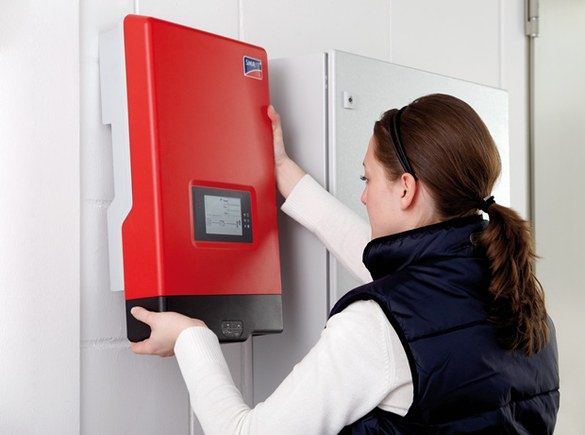
\includegraphics[width=0.5\linewidth]{../figures/SMA-Sunny-Boy.jpg}
%\\[0.5]
\caption{A domestic, grid connecting inverter from SMA. This is one of the many Sunny Boy models available}
\label{fig:SMA-inverter}
\end{figure}
\begin{itemize}
\item There are many brands such SMA and Fronius 
\item	The inverter changes DC to AC at the same frequency and voltage as the mains
\item	The inverter will monitor the mains before turning on and will reproduce the signal that the mains has
\item	For safety reasons the inverter must turn off very quickly if there is a power failure. If not the power lines on the PV side of any fault would be live.
\item	Grid tied inverters must meet strict standards of waveforms, safety etc
\item	Grid tied inverters often have displays, blue tooth links etc
\item	Costs vary but typically about \SI{1000}[\pounds]{}
\item	Life expectancy is apparently about 10 years
\item	The data sheet will state the number of input strings the inverter can accept and the max voltage on each string. 
\item	Grid tied inverters all have MPPT (maximum power point tracking). With MPPT the load that the inverter applies to the panels is changed such that the panels are always working at their maximum power output. The data sheet will give a range of voltages over which the MPPT will work. Use this and the data from the panels to establish how many modules can be in each string.
\item	Some inverters have connection for two or more strings but only one MPPT. Others have two or more MPPT devices, allowing for different strings to be working at completely different voltages. This is useful if a system is split between E and W facing roofs or if one area of the array might be shaded.
\item	Inverter efficiency drops dramatically at low output powers. For this reason the inverter is usually ‘undersized’ slightly or the right size but never ‘oversized’
\end{itemize}
\item \textbf{AC Isolator}
\begin{figure}[h]
\centering
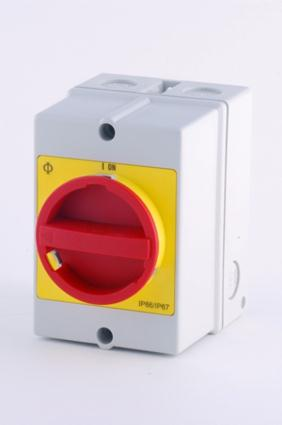
\includegraphics[width=0.25\linewidth]{../figures/AC-isolator.jpg}
%\\[0.5]
\caption{An AC isolator}
\label{fig:AC-isolator}
\end{figure}
\begin{itemize}
\item A big switch that will switch both the live and the neutral wires and cannot be turned on by accident – i.e. it ‘locks’ on or off. It is only necessary to have the AC Isolator between the inverter and the generation meter but the diagram above has two..
\end{itemize}
\item \textbf{Total generation meter}
\begin{figure}[ht]
\centering
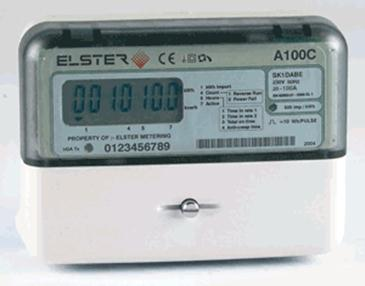
\includegraphics[width=0.25\linewidth]{../figures/TGM.jpg}
%\\[0.5]
\caption{A total generation meter}
\label{fig:TGM}
\end{figure}
\begin{itemize}
\item This measures the total energy generation of the panels. This meter reading is what the FIT payment is based on.
\end{itemize}
\item \textbf{Consumer Unit}
\begin{itemize}
\item This is the normal "fuse" board in the property
\end{itemize}
\item \textbf{Export meter}
\begin{itemize}
\item If this was in place, it would measure the energy exported to the national grid. The export tariff in the FIT scheme would be based on the reading from this meter.
\item Most energy suppliers will not bother with this meter but pay the export tariff based on a deemed export of 50\% of total generation. 
\end{itemize}
\item \textbf{Utility Meter}
\begin{itemize}
\item This is the normal meter in the property. If energy from the PV panels is used within the property then this meter records a lower value that it would if grid electricity was used instead. Some old fashioned meters will actually run backwards when exporting to the grid! It seems that energy companies are very slow to fix this so those with old meters get paid their export tariff but also have their meter reading reduced by the amount that they export!
\end{itemize}
\item \textbf{Fixings and cabling}
\begin{itemize}
\item Fixing to a roof is done by brackets which fix to the roof timbers under the tiles which support parallel tracks. The panels are bolted on to these tracks with wires run under the tiles or into the loft. 
\end{itemize}
\end{enumerate}

\section{The Effect of Location and Positioning of Panels}
\begin{itemize}
\item Shading has a very significant effect on output and should be avoided where possible.
\item Figure \ref{fig:op-vs-inclination} shows the impact of inclination on the annual output of a south facing  \SI{1}{\kilowattpeak} array located at St Agnes, Cornwall. The latitude of the location is \SI{50.3}{\degree\north} and the optimum inclination is about \SI{38}{\degree}, which is close to the angle of most roofs. It makes less than 5\% difference to the annual output if the inclination is as much as \SI{20}{\degree} steeper or more shallow than the optimum. A vertical panel would deliver about 30\% than one at optimal inclination, while a horizontal panel would deliver about 15\% less. However, panels that are inclined too close to the horizontal are more prone to collecting dirt, snow and other debris. The shading that results can have a very serious impact on annual output, as discussed above.

For comparison, the effect of varying inclinations are also shown for Abidjan, Ivory Coast (\SI{5.3}{\degree\north}) and Johannesburg, South Africa (\SI{26.2}{\degree\south}) 


\begin{figure}
\centering
\includegraphics[width=0.8\linewidth]{../figures/inclination-output.tex}
%\\[0.5]
\caption{The effect of inclination on the annual output of a \SI{1}{\kilowattpeak} array placed in Oslo, Norway,(\SI{60}{\degree\north}) St Agnes, Cornwall (\SI{53}{\degree\north}), Abidjan, Ivory Coast (\SI{5.3}{\degree\north}) and Johannesburg, South Africa (\SI{26.2}{\degree\south}). In each case the orientation is optimised for that location The data assume 7.7\% losses due to temperature and low irradiance, 3\% losses due to angular reflectance effects and other system losses in the inverter and cabling of 14\%, giving combined losses of 23\%.  \cite{PVGIS}}
\label{fig:op-vs-inclination}
\end{figure}

\item Figure shows the impact of orientation on a \SI{1}{\kilowattpeak} array at the optimal inclination for St Agnes, Cornwall.

\begin{figure}
\centering
\includegraphics[width=0.8\linewidth]{../figures/orientation-output.tex}
%\\[0.5]
\caption{Effect of orientation on an optiamlly inclided \SI{1}{\kilowattpeak} array in St Agnes, Cornwall.  \cite{PVGIS}}
\label{fig:op-vs-orientation}
\end{figure}

\end{itemize}
\begin{comment}
\begin{figure}[ht!]
     \begin{center}
%
        \subfigure[St Agnes \SI{53}{\degree\north}]{%
            \label{fig:first}
            \includegraphics[width=0.4\textwidth]{../figures/inclination-output.tex}
        }%
        \subfigure[St Agnes \SI{53}{\degree\north}]{%
           \label{fig:second}
           \includegraphics[width=0.4\textwidth]{../figures/inclination-output.tex}
        }\\ %  ------- End of the first row ----------------------%
        \subfigure[St Agnes \SI{53}{\degree\north}]{%
            \label{fig:third}
            \includegraphics[width=0.4\textwidth]{../figures/inclination-output.tex}
        }%
        \subfigure[St Agnes \SI{53}{\degree\north}]{%
            \label{fig:fourth}
            \includegraphics[width=0.4\textwidth]{../figures/inclination-output.tex}
        }%
%
    \end{center}
    \caption{%
        The l-o-n-g caption for all the subfigures
        (FirstFigure through FourthFigure) goes here.
     }%
   \label{fig:subfigures}
\end{figure}
\end{comment}

\section{Logistics of Buying, Installing and Connection}
\begin{itemize}
\item To qualify for the FIT, the installer must be MCS accredited (microgeneration certification scheme)
\item Costs for systems have dropped dramatically since the introduction of the FIT from £5000 / kWp a few years ago to something like £6000 for a 4kWp system now.
\item Costs cover scaffolding, design, site inspection, positioning panels and electrical equipment, connection, testing, communication with the DNO (district network operator, Western Power here), communication with local authority etc. as well as for the hardware that is purchased
\item The MCS publication “Photovoltaics in buildings – A guide to the installation of PV systems” \cite{MCS_PV_Guide} which is available on Moodle, sets out the standards that must be conformed to in the installation of solar pv. In particular it mentions G83/1 which is the standard for the connection of micro-generation systems of less than \SI{4}{\kilowattpeak}. Under this standard you only need to tell the DNO that you have connected the system on the day of installation i.e. no prior permission is necessary. The standards for larger systems require notification and permission from the DNO before connection can take place. 
\item Building Regulations approval is required for a PV installation – the MCS accredited installer will follow all correct procedures and then communicate with the local authority and building regs approval should follow without the need for inspection.
\item Planning permission may be needed although for many installations, especially those that are roof mounted, it is considered as a permitted change and is not.
\end{itemize}
\section{The Feed-in Tariff}
\begin{itemize}
\item	Electricity suppliers over a certain size are obliged to pay the FIT and export payments but the owner of the PV system can choose who they wish to pay their FIT. You are not obliged to enter into a contract with your electricity supplier for the FIT / export payments, but most people do.
\item	FIT is paid on the total generation of the system – normally there is a quarterly submission of the total generation meter reading which is followed by the FIT payment. 
\item	FIT is currently paid at two rates – a higher rate if the property is energy rating of band D or higher and a lower rate if the property is band E or lower, or if the property has never had an energy assessment
\item	Export payment is normally based on a deemed export of 50\% of the total generation.
\item	Savings on the consumer’s electricity bill vary depending on the pattern of energy use within the property. It would be reasonable to assume that something between 25\% and 50\% of the total generations would be used by the property and not exported to the grid – hence the property would expect its electricity bill to be this much smaller after installation of the PV.
\end{itemize}
\section{Estimate of annual output}
(for comparison, figures below relate to a \SI{2.35}{\kilowattpeak} roof mounted system on a roof of inclination \SI{25}{\degree} and azimuth \SI{-20}{\degree})
\begin{itemize}

\item	MCS accredited suppliers must give a quoted figure for the likely annual output and financial gains from a PV system. This figure is based on the 2005 SAP. For the \SI{2.35}{\kilowattpeak} considered here this was \SI{1890}{\kilowatthour} but the actual recorded output has been closer to \SI{2350}{\kilowatthour\per\year}.
\item	It is possible to treat the annual irradiation for the location as the ‘peak sun hours’. Here we receive about \SI{1230}{\kilowatthour\per\metre\squared\per\year}so we have 1230 peak sun hours – (i.e. the equivalent of 1230 hours of \SI{1000}{\watt\per\metre\squared}). This figure can be used with
\begin{itemize}
\item the area of the panels and the efficiency of the panels or better still
\item the peak power output of the panels (remember that they are tested at peak sun so for every hour of peak sun, the system should be giving out its peak power). A 2.35kWp system with 1230 peak sun hours should give an output of 2891kWh.  This is however the output of the panels and assumes that the panels are under test conditions. It is necessary to factor in losses for
\begin{itemize}
\item The inverter – which is probably about 90\% efficient overall
\item	The fact that panels will often be higher temp than the \SI{25}{\celsius} at which they are tested. (hotter panels give less energy output)
\item	The fact that the sun’s spectrum is not \SI{1.5}[AM]{} all year
\item	The fact that the radiation is striving the panels at an angle – reflections increase as the angle of incidence increases
\end{itemize}
\end{itemize}
For this reason it is appropriate to reduce the calculated output by something like 20\%, so for our example system we would expect $0.8 \times 1230 \times 2.35 = \SI{2312}{\kilowatthour}$.

\item	Software produced by manufacturers such as ‘Sunny Design’ which is free from SMA will provide estimates of system output, as well as helping with the specification of equipment such as inverters.
\item	There are several commercially available analysis tools such as ‘pvsol’ which will provide estimates of output. These tools can have detailed analysis of shading which can be useful.
\item	The simplest estimates come from pvgis \cite{PVGIS} gives very sensible estimations of the system output and has the facility to specify location, azimuth  and inclination. Outputs can be yearly, monthly or daily. There is a choice of pvgis-classic, which is based on ground based observations or pvgis-SAF which is based on satellite observations. (I find that the SAF prediction is closer than the classic, which is a bit low)
\item	As a rule of thumb, many people talk of the pv output in Cornwall being \SI{1000}{\kilowatthour} per kWp installed. For our example system, based on this rule, we should get 2350kWh per year. I have heard people say that for a well sited system, output can be up to \SI{1100}{\kilowatthour\per\kilowattpeak}
In reality, in the first 12 months after installation, our system generated \SI{2449}{\kilowatthour} (1042 kWh / kWp). Over the last 12 months it has generated \SI{2360}{\kilowatthour} (1004 kWh / kWp), with the highest ‘rolling’ 12 month figure being \SI{2467}{\kilowatthour} (1050 kWh / kWp) and the lowest at \SI{2283}{\kilowatthour} (971 kWh / kWp). 

\end{itemize}


\printbibliography

\end{document}
\begin{comment}
My system isn’t optimally positioned, and there is a very small amount of shading late in the evening, but even including that, it seems unlikely that a system would consistently generate at 1100 kWh / kWp – it is likely that an optimally positioned system would be generate about 1000kWh per kWp or greater over most years, so this is a reasonable estimate.  
\end{comment}